\documentclass[11pt, A4]{article}
%\usepackage[brazil]{babel}
\usepackage{graphicx}
\usepackage[utf8]{inputenc}
\usepackage[T1]{fontenc}
\usepackage{url}
\usepackage{Sweave}
\usepackage{natbib}
\usepackage{framed, color}
\usepackage{xspace}
\definecolor{shadecolor}{rgb}{0.9, 0.9, 0.9}
\setlength{\parindent}{0pt}
\setlength{\hoffset}{-0.5in}
\setlength{\textwidth}{6in}
\setlength{\voffset}{-0.1in}
%\pdfpagewidth=\paperwidth
%\pdfpageheight=\paperheight
\newcommand{\R}{\textnormal{\sffamily\bfseries R}\xspace}
% altered bc \sf is obsolete, see:
% http://tex.stackexchange.com/questions/74478/latex-command-incantation-for-r 
\newcommand{\code}[1]{\texttt{#1}}

%\VignetteIndexEntry{Introduction to sads}

\begin{document}

\title{Fitting species abundance models with maximum likelihood \\ Quick reference for \code{sads} package}
\author{Paulo In\'acio Prado,  Murilo Dantas Miranda and Andre Chalom \\ Theoretical Ecology Lab \\ LAGE at the Dep of Ecology, USP, Brazil \\ 
  %\url{http://ecologia.ib.usp.br/let/} \\
  \url{prado@ib.usp.br}}

\date{\today}

\maketitle


\section{Introduction}

Species abundance distributions (SADs) are one of the basic patterns
of ecological communities \citep{McGill2007}. 
The empirical distributions are
traditionally modeled through probability distributions. Hence, the
maximum likelihood method can be used to fit and compare competing
models for SADs. 
The package \code{sads} provides functions to fit the most used models
to empirical SADs. The resulting objects have methods to evaluate fits and compare competing
models. The package also allows the simulation of SADs expected from communities' 
samples, with and without aggregation of individuals of the same species.


\section{Installation}

The package is available on CRAN and can be installed in \R with the command:

\begin{Schunk}
\begin{Sinput}
> install.packages('sads')
\end{Sinput}
\end{Schunk}

then loaded by

\begin{Schunk}
\begin{Sinput}
> library(sads)
\end{Sinput}
\end{Schunk}

\subsection{Developer version}
\label{sec:developer-version}

The current developer version can be installed from GitHub with:

\begin{Schunk}
\begin{Sinput}
> library(devtools)
> install_github(repo = 'piLaboratory/sads', ref= 'dev', build_vignettes = TRUE)
\end{Sinput}
\end{Schunk}

And then load the package:

\begin{Schunk}
\begin{Sinput}
> library(sads)
\end{Sinput}
\end{Schunk}

\section{Exploratory analyses}
\label{sec:analise-exploratoria}

Throughout this document we'll use two data sets of abundances from the sads
package. For more information on these data please refer to their help
pages: 

\begin{Schunk}
\begin{Sinput}
> data(moths)# William's moth data used by Fisher et al (1943)
> data(ARN82.eB.apr77)# Arntz et al. benthos data
> data(birds)# Bird census used by Preston (1948)
\end{Sinput}
\end{Schunk}

\subsection{Octaves}
\label{sec:oitavas}

Function \code{octav} tabulates the number of species in classes
of logarithm of abundances at base 2 (Preston's octaves) and returns a data frame 
\footnote{actually an object of class \emph{octav} which inherits from class \emph{dataframe}}:

\begin{Schunk}
\begin{Sinput}
> (moths.oc <- octav(moths))
\end{Sinput}
\begin{Soutput}
Object of class "octav"
   octave upper Freq
1       0     1   35
2       1     2   11
3       2     4   29
4       3     8   32
5       4    16   26
6       5    32   32
7       6    64   31
8       7   128   13
9       8   256   19
10      9   512    5
11     10  1024    6
12     11  2048    0
13     12  4096    1
14     13  8192    0
\end{Soutput}
\begin{Sinput}
> (arn.oc <- octav(ARN82.eB.apr77))
\end{Sinput}
\begin{Soutput}
Object of class "octav"
   octave      upper Freq
1      -7 7.8125e-03    0
2      -6 1.5625e-02    3
3      -5 3.1250e-02    5
4      -4 6.2500e-02    4
5      -3 1.2500e-01    6
6      -2 2.5000e-01    3
7      -1 5.0000e-01    5
8       0 1.0000e+00    2
9       1 2.0000e+00    4
10      2 4.0000e+00    3
11      3 8.0000e+00    1
12      4 1.6000e+01    2
13      5 3.2000e+01    0
14      6 6.4000e+01    1
15      7 1.2800e+02    1
16      8 2.5600e+02    0
\end{Soutput}
\end{Schunk}

A logical argument \code{preston} allows smoothing the numbers as proposed by \citet{Preston1948}. 

The octave number is the upper limit of the class in log2 scale. 
Hence, for abundance values smaller than one (\emph{e.g.} biomass data) the octave numbers are negative.
A Preston plot is a histogram of this table, obtainable by applying the function \code{plot} to the data frame:

\setkeys{Gin}{width=0.65\textwidth}

{\centering
\begin{Schunk}
\begin{Sinput}
> plot(moths.oc)
\end{Sinput}
\end{Schunk}
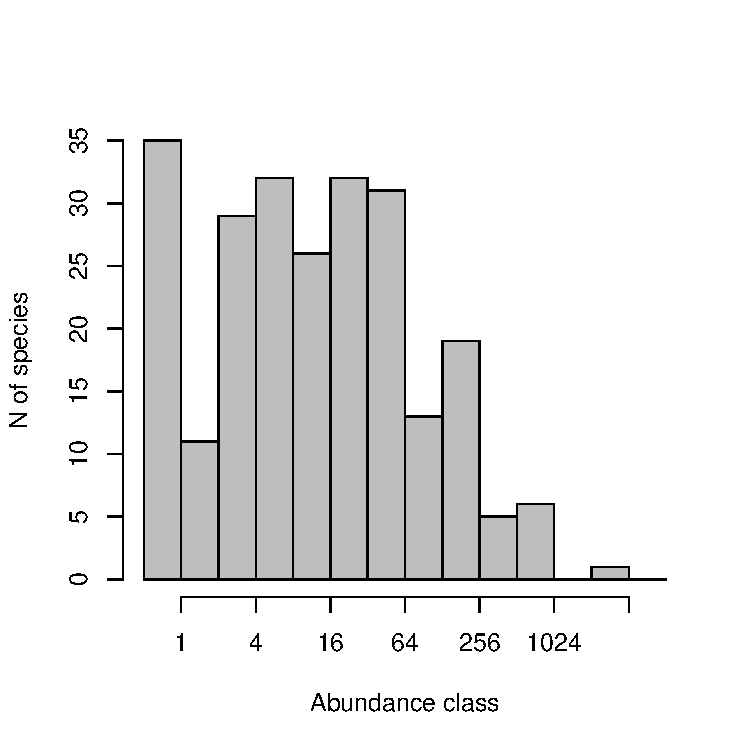
\includegraphics{sads_intro-woven-Ploting-octaves}
}

{\centering
\begin{Schunk}
\begin{Sinput}
> plot(arn.oc)
\end{Sinput}
\end{Schunk}
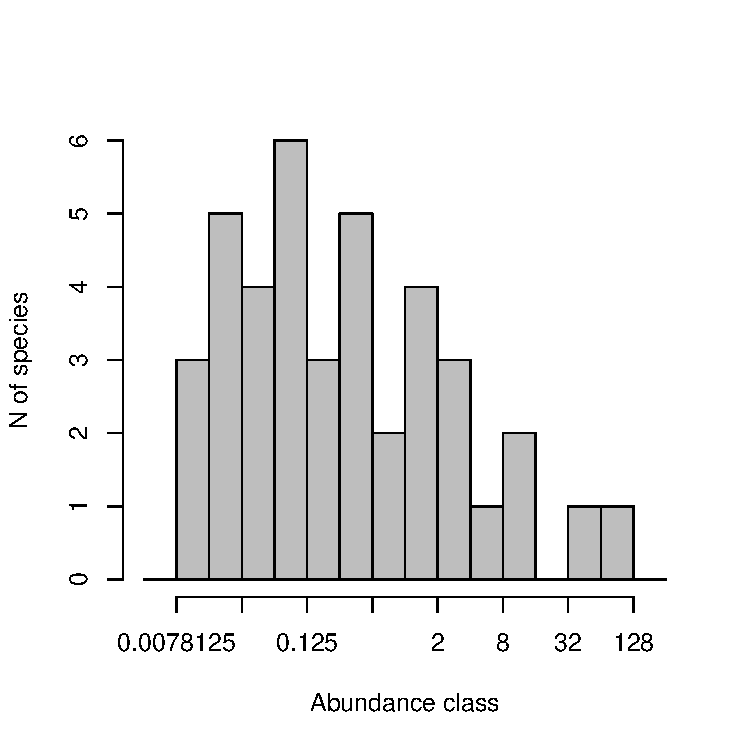
\includegraphics{sads_intro-woven-Biomass-octave-plot}
}

The plot method for objects of class \code{octav} has 
a logical argument \code{prop} that rescales the y-axis to relative frequencies of species in each octave,
which can be used to compare different data sets:

\begin{Schunk}
\begin{Sinput}
> plot(moths.oc, prop = TRUE, border=NA, col=NA)
> lines(octav(birds), mid = FALSE, prop = TRUE, col="red")
> lines(octav(moths), mid = FALSE, prop = TRUE)
> legend("topright", c("Preston's birds", "Fisher's moths"), col=c("red", "blue"), lty=1, bty="n")
\end{Sinput}
\end{Schunk}


\subsection{Rank-abundance plots}
\label{sec:rank_abund}
Function \code{rad} returns a data frame of sorted abundances and their ranks 
\footnote{actually an object of class \emph{rad} which inherits from class \emph{dataframe}}:

\begin{Schunk}
\begin{Sinput}
> head(moths.rad <- rad(moths))
\end{Sinput}
\begin{Soutput}
  rank abund
1    1  2349
2    2   823
3    3   743
4    4   604
5    5   589
6    6   572
\end{Soutput}
\begin{Sinput}
> head(arn.rad <- rad(ARN82.eB.apr77))
\end{Sinput}
\begin{Soutput}
     rank abund
sp17    1 67.21
sp11    2 54.67
sp33    3 14.67
sp9     4  9.90
sp30    5  5.71
sp10    6  2.88
\end{Soutput}
\end{Schunk}

To get the rank-abundance or Whitaker's plot apply the function \code{plot} on the data frame:

\setkeys{Gin}{width=0.65\textwidth}
{\centering % centers BOTH of the next plots
\begin{Schunk}
\begin{Sinput}
> plot(moths.rad, ylab="Number of individuals")
\end{Sinput}
\end{Schunk}
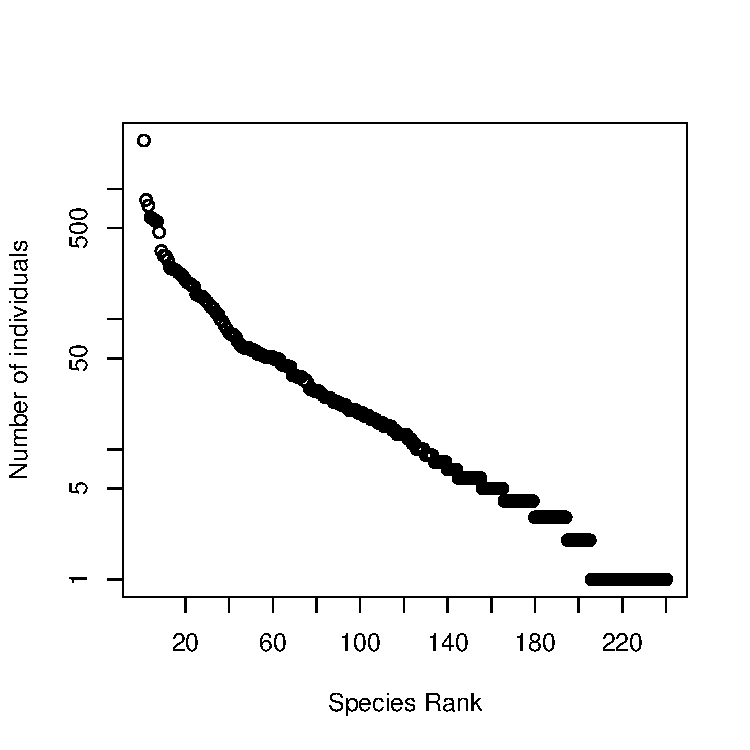
\includegraphics{sads_intro-woven-radplot1}
}

{\centering
\begin{Schunk}
\begin{Sinput}
> plot(arn.rad, ylab="Biomass")
\end{Sinput}
\end{Schunk}
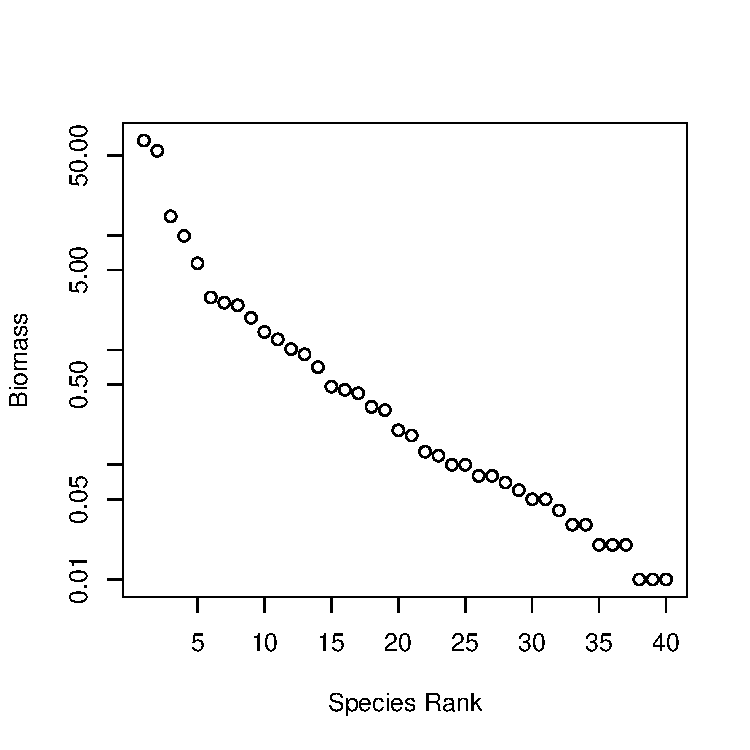
\includegraphics{sads_intro-woven-radplots}
}

Again, the plot method for \code{rad}  has a logical argument \code{prop} 
rescales the y-axis to depict relative abundances:

\begin{Schunk}
\begin{Sinput}
> plot(moths.rad, prop = TRUE, type="n")
> lines(rad(birds), prop = TRUE, col="red")
> lines(rad(moths), prop = TRUE)
> legend("topright", c("Preston's birds", "Fisher's moths"), col=c("red", "blue"), lty=1, bty="n")
\end{Sinput}
\end{Schunk}

\section{Model fitting}
\label{sec:ajuste-e-selecao}
The \emph{sads} package provides maximum-likelihood fits of many
probability distributions to empirical sads. The working horses are the
functions \code{fitsad} for fitting species abundance distributions
and \code{fitrad} for fitting rank-abundance distributions. The first
argument of these functions is the vector of observed abundances 
\footnote{\code{fitrad} also accepts a rank-abundance table returned by function \code{rad} as its first argument.} 
The second argument is the name of the model to be fitted.
Please refer to the help
page of the functions for details on the models. For more information
on the fitting procedure see also the vignette of
the \emph{bbmle} package, on top of which the package \emph{sads} is built.

To fit a log-series distribution use the argument \code{sad='ls'}:

\begin{Schunk}
\begin{Sinput}
> (moths.ls <- fitsad(moths,'ls'))
\end{Sinput}
\begin{Soutput}
Maximum likelihood estimation
Type: discrete  species abundance distribution
Species: 240 individuals: 15609 

Call:
mle2(minuslogl = function (N, alpha) 
-sum(dls(x, N, alpha, log = TRUE)), start = list(alpha = 40.247281791951), 
    method = "Brent", fixed = list(N = 15609L), data = list(x = list(
        1, 1, 1, 1, 1, "etc")), lower = 0, upper = 240L)

Coefficients:
          N       alpha 
15609.00000    40.24728 

Log-likelihood: -1087.71 
\end{Soutput}
\end{Schunk}

The resulting model object inherits from \emph{mle2}
\citep{Bolkerbbmle}, and has all usual methods for model objects, such as
summaries, log-likelihood, and AIC values:
\begin{Schunk}
\begin{Sinput}
> summary(moths.ls)
\end{Sinput}
\begin{Soutput}
Maximum likelihood estimation

Call:
mle2(minuslogl = function (N, alpha) 
-sum(dls(x, N, alpha, log = TRUE)), start = list(alpha = 40.247281791951), 
    method = "Brent", fixed = list(N = 15609L), data = list(x = c(1L, 
    1L, 1L, 1L, 1L, 1L, 1L, 1L, 1L, 1L, 1L, 1L, 1L, 1L, 1L, 1L, 
    1L, 1L, 1L, 1L, 1L, 1L, 1L, 1L, 1L, 1L, 1L, 1L, 1L, 1L, 1L, 
    1L, 1L, 1L, 1L, 2L, 2L, 2L, 2L, 2L, 2L, 2L, 2L, 2L, 2L, 2L, 
    3L, 3L, 3L, 3L, 3L, 3L, 3L, 3L, 3L, 3L, 3L, 3L, 3L, 3L, 3L, 
    4L, 4L, 4L, 4L, 4L, 4L, 4L, 4L, 4L, 4L, 4L, 4L, 4L, 4L, 5L, 
    5L, 5L, 5L, 5L, 5L, 5L, 5L, 5L, 5L, 6L, 6L, 6L, 6L, 6L, 6L, 
    6L, 6L, 6L, 6L, 6L, 7L, 7L, 7L, 7L, 7L, 8L, 8L, 8L, 8L, 8L, 
    8L, 9L, 9L, 9L, 9L, 10L, 10L, 10L, 10L, 11L, 11L, 12L, 12L, 
    13L, 13L, 13L, 13L, 13L, 14L, 14L, 15L, 15L, 15L, 15L, 16L, 
    16L, 16L, 17L, 17L, 17L, 18L, 18L, 18L, 19L, 19L, 19L, 20L, 
    20L, 20L, 20L, 21L, 22L, 22L, 22L, 23L, 23L, 23L, 24L, 25L, 
    25L, 25L, 26L, 27L, 28L, 28L, 28L, 29L, 29L, 32L, 34L, 34L, 
    36L, 36L, 36L, 37L, 37L, 43L, 43L, 44L, 44L, 45L, 49L, 49L, 
    49L, 51L, 51L, 51L, 51L, 52L, 53L, 54L, 54L, 57L, 58L, 58L, 
    60L, 60L, 60L, 61L, 64L, 67L, 73L, 76L, 76L, 78L, 84L, 89L, 
    96L, 99L, 109L, 112L, 120L, 122L, 129L, 135L, 141L, 148L, 
    149L, 151L, 154L, 177L, 181L, 187L, 190L, 199L, 211L, 221L, 
    226L, 235L, 239L, 244L, 246L, 282L, 305L, 306L, 333L, 464L, 
    560L, 572L, 589L, 604L, 743L, 823L, 2349L)), lower = 0, upper = 240L)

Coefficients:
      Estimate Std. Error z value     Pr(z)    
alpha   40.247      6.961  5.7818 7.391e-09 ***
---
Signif. codes:  
0 ‘***’ 0.001 ‘**’ 0.01 ‘*’ 0.05 ‘.’ 0.1 ‘ ’ 1

Fixed parameters:
    N 
15609 

-2 log L: 2175.425 
\end{Soutput}
\begin{Sinput}
> coef(moths.ls)
\end{Sinput}
\begin{Soutput}
          N       alpha 
15609.00000    40.24728 
\end{Soutput}
\begin{Sinput}
> logLik(moths.ls)
\end{Sinput}
\begin{Soutput}
'log Lik.' -1087.713 (df=1)
\end{Soutput}
\begin{Sinput}
> AIC(moths.ls)
\end{Sinput}
\begin{Soutput}
[1] 2177.425
\end{Soutput}
\end{Schunk}

On the above examples, notice that the \code{print} method\footnote{Or, equivalently, the \code{show} method}
displays some statistics on the input data and 
fitting function used - number of species, number of individuals, truncation point for the probability 
distribution (when used, see below) and whether we are fitting a discrete or
continuous sad or rad - while the \code{summary} method displays information more associated with the
fitting \emph{per se}: standard errors and significance codes for each parameter. Also, notice that
the input data is displayed by both methods, but the \code{print} method only shows the first values, as the
complete list can be quite large.

\subsection{Model diagnostics}
\label{sec:model-diagnostics}
Many other diagnostic and functions are available for sad and rad models. 
To get likelihood profiles, likelihood intervals and confidence intervals use:

\setkeys{Gin}{width=\textwidth}

\begin{Schunk}
\begin{Sinput}
> moths.ls.prf <- profile(moths.ls)
> likelregions(moths.ls.prf) #likelihood intervals
\end{Sinput}
\begin{Soutput}
Likelihood regions for ratio = 2.079442 

 alpha:
        lower    upper
[1,] 27.57325 56.04053
\end{Soutput}
\begin{Sinput}
> confint(moths.ls.prf)
\end{Sinput}
\begin{Soutput}
   2.5 %   97.5 % 
28.01537 55.36267 
\end{Soutput}
\end{Schunk}

Then use \code{plotprofmle} to plot likelihood profiles at the original scale (relative negative log-likelihood)
and function \code{plot} to get plots at chi-square scale (square-root of twice the relative log-likelihood):

\setkeys{Gin}{width=\textwidth}

\begin{Schunk}
\begin{Sinput}
> par(mfrow=c(1,2))
> plotprofmle(moths.ls.prf)# log-likelihood profile
> plot(moths.ls.prf)# z-transformed profile
> par(mfrow=c(1,1))
\end{Sinput}
\end{Schunk}
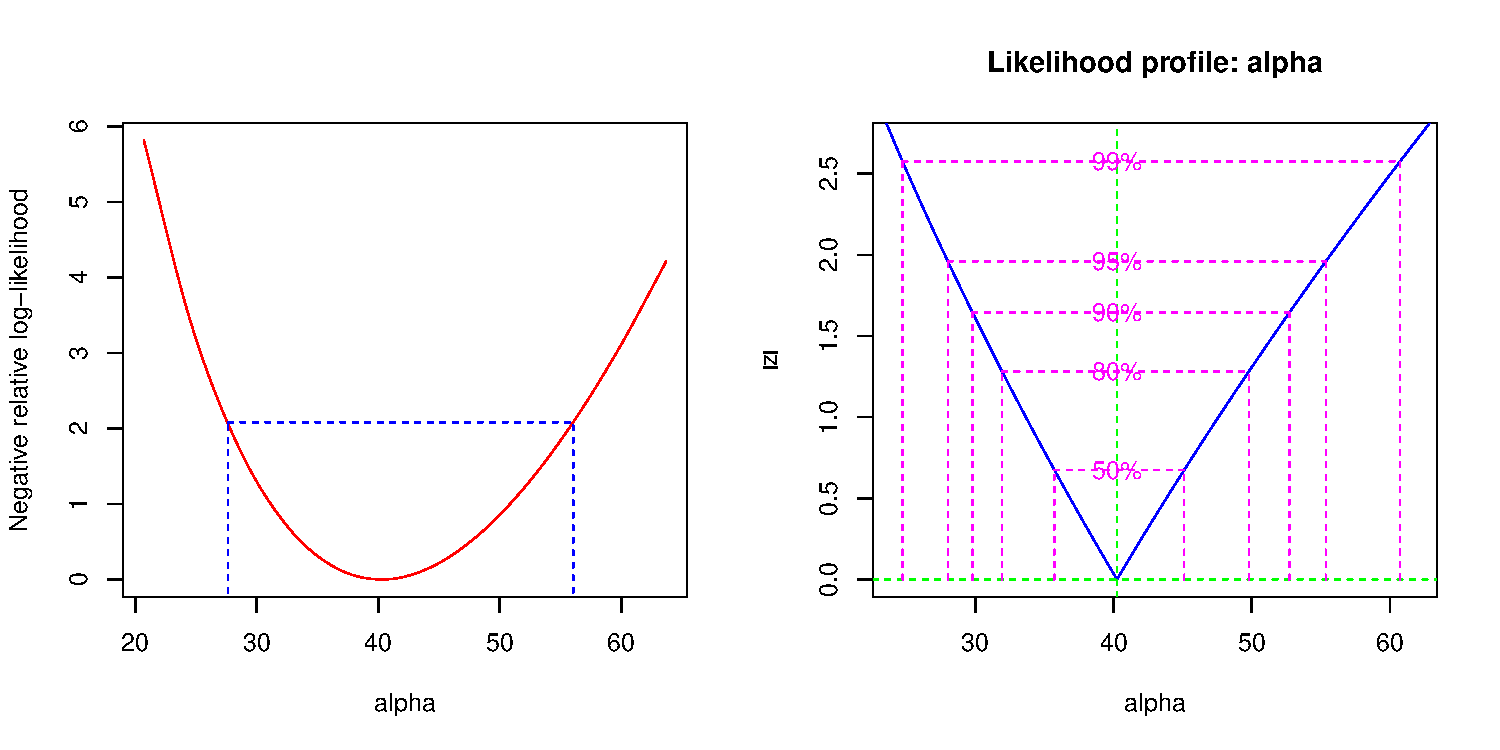
\includegraphics{sads_intro-woven-Ploting-profiles}

\begin{shaded}
  \textbf{Likelihood intervals and confindence intervals:} \hfill
  Likelihood intervals include all values of the parameters that have up to a given 
  log-likelihood absolute difference to the maximum likelihood estimate.
  This difference is the log-likelihood ratio and is set with the argument \code{ratio} 
  of function \code{likelregions}. The default value of \code{ratio} is log(8), and thus
  in the example above the likelihood interval encloses all values of the parameter 
  that are up to 8 times as plausible
  as the estimated value of $\alpha = $ 40.25.
  
  Likelihood intervals at log(8) converge to the value of confidence intervals at 95\%
  as sample size increases. In most cases even for moderate sample sizes the limits of
  confidence and likelihood intervals are very close. Discrepancies occur only when the likelihood profile
  is highly asymmetric or have local {\em minima}. But in this kind of profile usually indicates an ill-behaved
  fit, and so the intervals may not be meaningful anyway.
\end{shaded}


When applied on a sad model object, the function \code{plot} returns four diagnostic plots:
\begin{Schunk}
\begin{Sinput}
> par(mfrow=c(2,2))
> plot(moths.ls)
> par(mfrow=c(1,1))
\end{Sinput}
\end{Schunk}
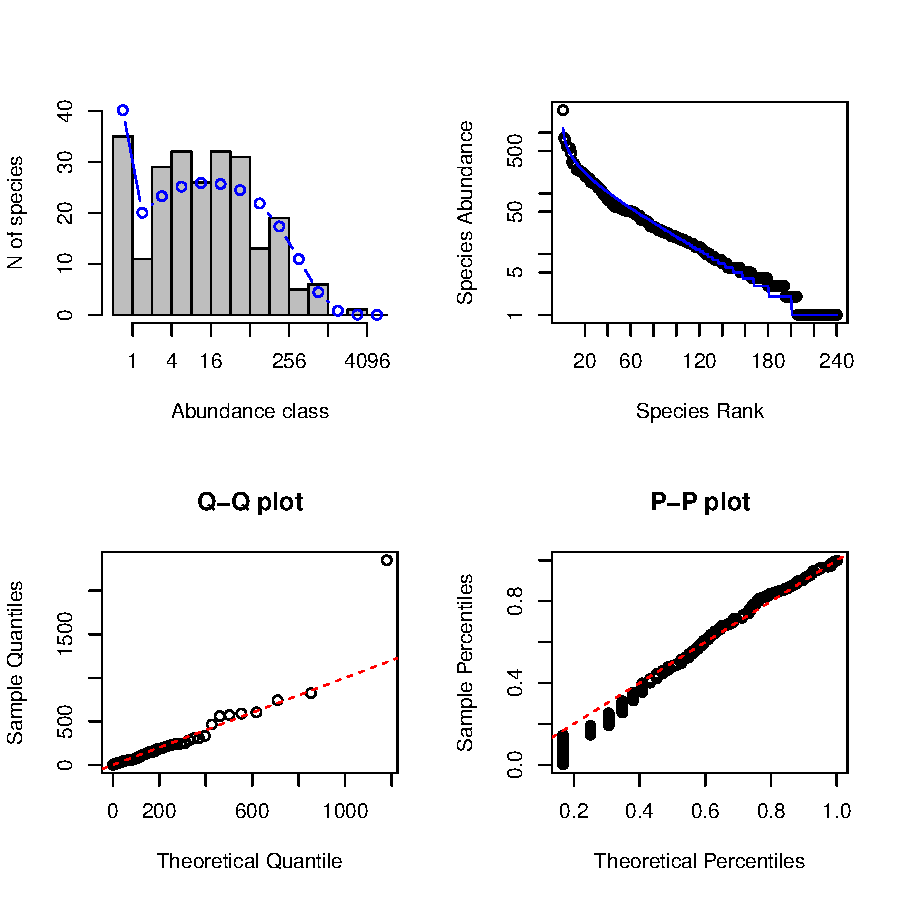
\includegraphics{sads_intro-woven-Plot-of-predicted-values}


The first two plots (top right and left) are the octave and rank-abundance plots with the predicted values 
of number of species in each octave 
and of each species' abundance. The two last plots (bottom) are quantile-quantile and percentile-percentile graphs of 
the observed vs. predicted abundances. The straight line indicates the expected relation in case of perfect fit.

\subsection{SADs vs RADs}

Species-abundance models assign a probability for each abundance
value. Thus, these models are probability density functions (PDFs) of
abundances of species. 
Rank-abundance models assign a probability for each
\textbf{abundance rank}. They are PDFs for rankings of species. The models are
interchangeable \citep{May1975}, but currently only four rad models
are available in package sads through the argument \code{rad} of
function \code{fitrad}:

\begin{itemize}
\item ``gs'': geometric series (which is NOT geometric PDF, available
  in \code{fitsad} as ``geom'')
\item ``rbs'': broken-stick model \citep{macarthur1957, May1975}
\item ``zipf'': Zipf power-law distribution
\item ``mand'': Zipf-Mandelbrot power-law distribution
\end{itemize}

\begin{shaded}
  \textbf{Comparison to \code{radfit} from \emph{vegan} package:} \hfill
  
  fits by \code{fitsad}, \code{fitrad} and \code{radfit} of \emph{vegan} 
  package provide similar estimates of model coefficients 
  but not comparable likelihood values. The reason for this is the fact each function fits models that assign 
  probability values to data in different ways. Function \code{fitsad} fits PDFs to observed abundances and \code{fitrad} fits PDFs 
  to the ranks of the abundances. Finally, \code{radfit} of \emph{vegan} fits a Poisson generalized linear model 
  to the \emph{expected abundances} deduced 
  from rank-abundance relationships from the corresponding sads and rads models \citep{wilson1991}. 
  See also the help page of \code{radfit}. 
  Therefore \textbf{likelihoods obtained from these three functions are not comparable}.
\end{shaded}

\section{Model selection}

It's possible to fit other models to the same data set, such as the Poisson-lognormal and a truncated lognormal:
\begin{Schunk}
\begin{Sinput}
> (moths.pl <- fitsad(x=moths, sad="poilog"))#default is zero-truncated
\end{Sinput}
\begin{Soutput}
Maximum likelihood estimation
Type: discrete  species abundance distribution
Species: 240 individuals: 15609 

Call:
mle2(minuslogl = function (mu, sig) 
-sum(dtrunc("poilog", x = x, coef = list(mu = mu, sig = sig), 
    trunc = trunc, log = TRUE)), start = list(mu = 1.99664912324681, 
    sig = 2.18726037265132), data = list(x = list(1, 1, 1, 1, 
    1, "etc")))

Coefficients:
      mu      sig 
1.996463 2.187131 

Truncation point: 0 

Log-likelihood: -1086.07 
\end{Soutput}
\begin{Sinput}
> (moths.ln <- fitsad(x=moths, sad="lnorm", trunc=0.5)) # lognormal truncated at 0.5
\end{Sinput}
\begin{Soutput}
Maximum likelihood estimation
Type: continuous  species abundance distribution
Species: 240 individuals: 15609 

Call:
mle2(minuslogl = function (meanlog, sdlog) 
-sum(dtrunc("lnorm", x, coef = list(meanlog = meanlog, sdlog = sdlog), 
    trunc = trunc, log = TRUE)), start = list(meanlog = 2.57905878609957, 
    sdlog = 1.78235276032689), data = list(x = list(1, 1, 1, 
    1, 1, "etc")))

Coefficients:
 meanlog    sdlog 
2.274346 2.039740 

Truncation point: 0.5 

Log-likelihood: -1086.36 
\end{Soutput}
\end{Schunk}

moreover, the function \code{AICtab} and friends from the \emph{bbmle} package can be used to get a model selection table:

\begin{Schunk}
\begin{Sinput}
> AICtab(moths.ls, moths.pl, moths.ln, base=TRUE)
\end{Sinput}
\begin{Soutput}
         AIC    dAIC   df
moths.pl 2176.1    0.0 2 
moths.ln 2176.7    0.6 2 
moths.ls 2177.4    1.3 1 
\end{Soutput}
\end{Schunk}

\textbf{NOTICE} that the information criterion methods do not differentiate between
\code{fitsad} and \code{fitrad} methods. Because of this, it is possible to include
\code{fitsad} and \code{fitrad} objects in the same IC-table without generating an error,
but the result will be meaningless.

To compare visually fits first get octave tables:

\begin{Schunk}
\begin{Sinput}
> head(moths.ls.oc <- octavpred(moths.ls))
\end{Sinput}
\begin{Soutput}
  octave upper     Freq
1      0     1 40.14377
2      1     2 20.02026
3      2     4 23.27123
4      3     8 25.12674
5      4    16 25.86285
6      5    32 25.67116
\end{Soutput}
\begin{Sinput}
> head(moths.pl.oc <- octavpred(moths.pl))
\end{Sinput}
\begin{Soutput}
  octave upper     Freq
1      0     1 27.58748
2      1     2 19.48221
3      2     4 26.76474
4      3     8 31.88373
5      4    16 33.16136
6      5    32 30.49056
\end{Soutput}
\begin{Sinput}
> head(moths.ln.oc <- octavpred(moths.ln))
\end{Sinput}
\begin{Soutput}
  octave upper     Freq
1      0     1 15.41886
2      1     2 22.44066
3      2     4 29.13034
4      3     8 33.72746
5      4    16 34.82976
6      5    32 32.08088
\end{Soutput}
\end{Schunk}

then use \code{lines} to superimpose the predicted values on the octave plot:

\setkeys{Gin}{width=0.75\textwidth}
\begin{Schunk}
\begin{Sinput}
> plot(moths.oc)
> lines(moths.ls.oc, col="blue")
> lines(moths.pl.oc, col="red")
> lines(moths.ln.oc, col="green")
> legend("topright", 
        c("Logseries", "Poisson-lognormal", "Truncated lognormal"), 
        lty=1, col=c("blue","red", "green"))
\end{Sinput}
\end{Schunk}
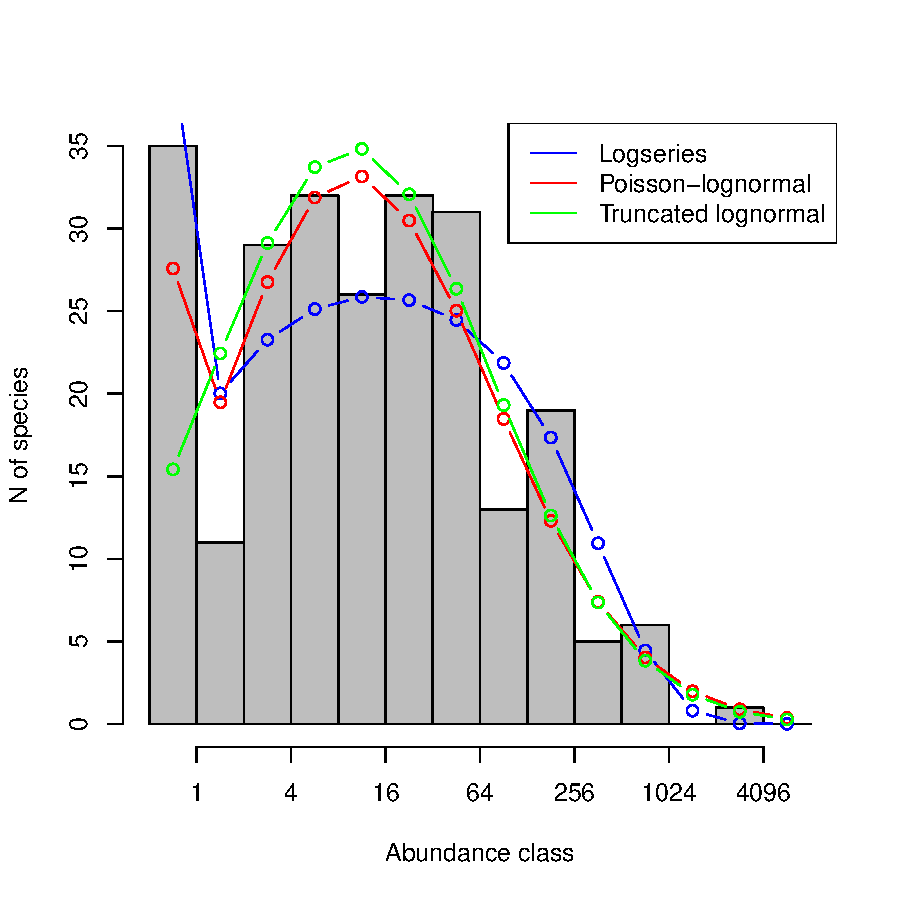
\includegraphics{sads_intro-woven-Octaves-plot}

To do the same with rank-abundance plots get the rank-abundance objects:

\begin{Schunk}
\begin{Sinput}
> head(moths.ls.rad <- radpred(moths.ls)) 
\end{Sinput}
\begin{Soutput}
  rank abund
1    1  1180
2    2   854
3    3   710
4    4   619
5    5   554
6    6   503
\end{Soutput}
\begin{Sinput}
> head(moths.pl.rad <- radpred(moths.pl))
\end{Sinput}
\begin{Soutput}
  rank abund
1    1  4348
2    2  1973
3    3  1322
4    4  1001
5    5   807
6    6   676
\end{Soutput}
\begin{Sinput}
> head(moths.ln.rad <- radpred(moths.ln))
\end{Sinput}
\begin{Soutput}
  rank     abund
1    1 3524.2394
2    2 1674.8603
3    3 1148.3539
4    4  883.6309
5    5  720.7864
6    6  609.2707
\end{Soutput}
\end{Schunk}

then plot observed and predicted values:

\begin{Schunk}
\begin{Sinput}
> plot(moths.rad)
> lines(moths.ls.rad, col="blue")
> lines(moths.pl.rad, col="red")
> lines(moths.ln.rad, col="green")
> legend("topright", 
        c("Logseries", "Poisson-lognormal", "Truncated lognormal"), 
        lty=1, col=c("blue","red", "green"))
\end{Sinput}
\end{Schunk}
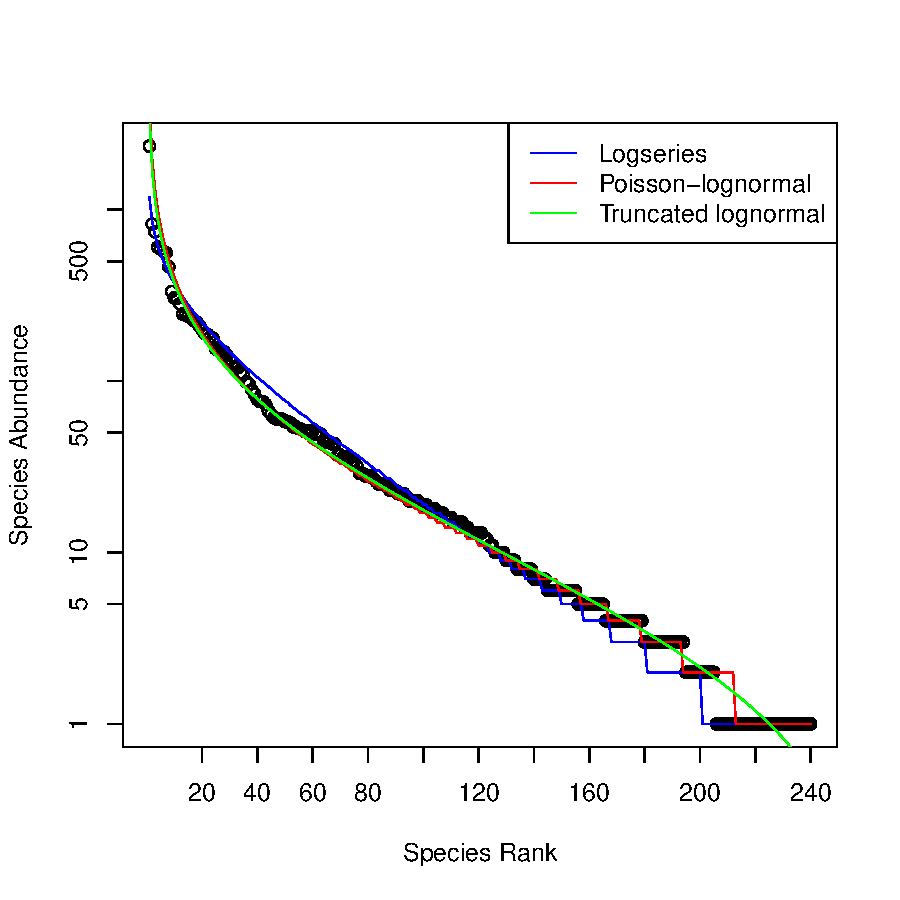
\includegraphics{sads_intro-woven-Rad-plots}

\subsection{Abundance class data}

For ecological communities, the representation of species abundances
typically occurs through categorization. For instance, when assessing
the abundance of sessile organisms, it is common practice to utilize a
scale based on the coverage of sampling areas, beacause direct enumeration
of individuals or estimation of biomass are  are extremely laborious.

The package \code{sads} has a specific class for fitting continuous
distributions for this kind of data. We will show the use of this
class using the data from \citet{Vieira2020}, who provide the coverage
class of each plant species in plots set in grasslands in
Southern Brazil. The object \code{grasslands} has the data from plot
'CA8', which has the largest number of species recorded in this study.

\begin{Schunk}
\begin{Sinput}
> head(grasslands)